\documentclass[11pt, a4paper]{report}
\usepackage{graphicx}
\usepackage[table,xcdraw]{xcolor}
\usepackage{geometry}
\usepackage{float}
\usepackage{authblk}
\usepackage{anyfontsize}
\usepackage[document]{ragged2e}
\usepackage{titlesec}
\usepackage[parfill]{parskip}
\usepackage{color}   %May be necessary if you want to color links
\usepackage{hyperref}
\usepackage{caption}
\usepackage{tabularx}
\usepackage{longtable}
\usepackage{blindtext}
\usepackage{pdflscape}
\hypersetup{
    colorlinks=true, %set true if you want colored links
    linktoc=all,     %set to all if you want both sections and subsections linked
    linkcolor=black,  %choose some color if you want links to stand out
}
\titleformat{\chapter}[hang] 
{\normalfont\huge\bfseries}{\chaptertitlename\ \thechapter:}{1em}{} 
\geometry{left=2.5cm,right=2.5cm,top=2.5cm,bottom=2.5cm}
\graphicspath{ {./images/} }


% Handy link: https://artofproblemsolving.com/wiki/index.php/LaTeX:Layout

% CHECK https://www.youtube.com/watch?v=ZYvS52511oQ FOR INFO ON SETTINGS FOR biblatex


\begin{document}
\pagestyle{empty}
\centering
\fontsize{2cm}{2cm}\selectfont{Plan of Approach} \\
\vspace{2mm}
\fontsize{1cm}{1cm}\selectfont Hardware Simulator \\
\vspace{2mm}
\large Project S7\\
\normalsize
\vspace{4cm}
% \includegraphics[width=\linewidth]{3DR_P1_Perspective.png}\\
\vfill
\normalsize Hein Verhallen \\
Nikola Panchev \\
Robin van den Dungen \\
Wyatt Southard \\
Youri Tils \\
Fontys Hogescholen, De Rondom 1, 5612 AP Eindhoven \\
\today

\begin{justify}


\newpage
\tableofcontents
\thispagestyle{empty}

\listoffigures
\thispagestyle{empty}


\listoftables
\thispagestyle{empty}

\newpage
\pagestyle{plain}
\setcounter{page}{1}

\chapter*{Abbreviation List}

\begin{table}[!h]
	\centering
\begin{tabular}{|c|c|}
	\hline
\textbf{Abbreviation} & \textbf{Explanation}        \\ \hline
BMS                   & Battery management system    \\ \hline
Li-ion	              & Lithium-ion    \\ \hline
\end{tabular}
\caption{List of commonly used Abbreviations}
\label{Abbreviation list}
\end{table}

\chapter{Background}
	\IEEEPARstart
{E}{nergy} storage is one of the grand technological challenges posed by the transformation from a
fossil fuel dependent society to one that relies on renewable energy sources. Batteries provide
some good solutions to these challenges, however, the present battery technologies suffer from
high weight, short lifetime, long charging time and limited safety.

The BatteryNL consortium is focused on developing the next generation of more efficient
batteries with enhanced performance. Fontys Engineering is helping BatteryNL with the development 
of an optimized battery management system (BMS), testing which can be quite
hazardous. Modern batteries can store a lot of energy, and if they catch fire, can be difficult to
extinguish. In addition to that, an insufficiently tested BMS can pose a hazard to users and to
the environment.

The solution to that is to emulate the battery and the load, so that testing can be completed
under a wide range of conditions without taking excessive risks.

This document explains in detail the development process of this project. 
Architecture, hardware, software, testing and results are covered for every design 
iteration of the process. 

The design is based on the 14-cell slider battery pack emulator kit by 
NXP \cite{UM11349}.

\chapter{Project result}
	\begin{figure}[ht]
    \centering
    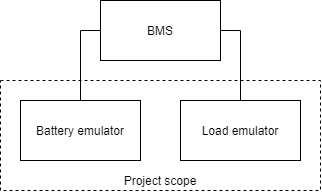
\includegraphics[scale=0.7]{System_context_diagram.png}
    \caption{System context diagram}
    \label{fig:system_context_diagram}
\end{figure}

The goal of this project is to design, built and test a battery pack emulator and (optionally) a load emulator that can be used to test a BMS (see figure \ref{fig:system_context_diagram}). This battery pack emulator should in the first design iteration be capable of emulating a battery pack with Li-ion cell characteristics. In order to emulate a Li-ion cell correctly it should be possible to emulate both charging and discharging of the Li-ion cell. 

Because the project team members are not yet experts in the field of designing battery pack emulators for BMS testing, it is chosen to design the battery pack emulator in iterations. In the first design iteration a battery pack emulator circuit will be designed which emulates the characteristics of a Li-ion battery pack. This battery pack emulator consists of two Li-ion cell emulators which are capable of charging and discharging. The voltages of each emulated cell are adjusted by a mechanical variable resistor. Each emulated cell has a voltage and current range that is 20\% larger than the safe operating area of a Li-ion cell.

In the second design iteration software will be added to the battery emulator circuit to control the voltages of each emulated cell via software. Also the temperature will be emulated in the battery pack emulator. The third design iteration consists of expanding the amount of emulated cells in the emulated battery pack to 14 cells. In the fourth design iteration a load emulator will be designed to test the BMS under different load conditions. This load emulator is capable of emulating electronics and motors. 

% The goal of this project is to design a programmable hardware system that presents a BMS with a "battery" and a "load" (see figure \ref{fig:system_context_diagram}). The hardware system emulates the battery and load. By using only software changes the hardware system should be able to emulate a battery with a different chemistry, capacity and cell topology. Likewise the hardware system should be able to emulate different loads from electronics through to motors under varying load.

At the end of the project it is expected that a battery pack emulator and optionally a load emulator is delivered. And if the planning allows it, a research report on existing battery and load emulators and the requirements for future battery and load emulators is delivered.

\section{Research questions}
In order to acquire functional requirements the following research questions have been derived:
% To be able to accomplish these deliverables the following research questions have been derived:
\begin{itemize}
    \item What is the safe operating area for Li-ion cells?
    % \item What different battery chemistries are there?
    % \item How do different battery chemistries behave?
    % \item What different battery cell topologies are there?
    % \item How do different battery cell topologies behave?
    % \item How do different battery capacities behave?
    % \item What kind of loads are there?
    % \item How do different loads behave?
    % \item How to control the voltage, current and phase to emulate a battery cell via software changes?
    % \item How to control the voltage, current and phase to emulate a load via software changes?
    \item How do existing battery emulators work?
    \item How do existing load emulators work?
    % \item What are the requirements for future emulators?
\end{itemize}

\section{Requirements}
For this project the following non-functional requirements with their functional requirements have been specified (see Appendix).

  
  
% \end{longtable}

% \begin{longtable}{|c|p{10cm}|c|c|}
%     \hline
%     \textbf{ID} & \textbf{Requirement} & \textbf{Priority} & \textbf{Status}\\ \hline 
%     \textbf{U1} & The hardware is able to emulate a battery with a specific lithium-ion chemistry and capacity & Must & Proposed\\ \hline
%     \textbf{U2} & The hardware is flexible enough to require only software changes to emulate a battery with a different chemistry, a different capacity, and a different cell topology & Must & Proposed\\ \hline
%     % \textbf{U3} & The hardware is able to emulate different loads: from electronics through to motors under varying load & Must & Proposed\\ \hline
%     \textbf{U3} & The hardware system is able to adjust the load impedance characteristic curve & Must & Proposed\\ \hline
%     % \textbf{U4} & The hardware system is tested & Must & Proposed\\ \hline
%     \textbf{U4} & The hardware is able to control the voltage, current and phase independently & Must & Proposed\\ \hline
%     \textbf{U5} & The hardware contains a BMS & Won't & Proposed\\ \hline
% \end{longtable}




	
\chapter{Project activities}
	This chapter will detail the activies that will take place during the project and are listed below. 

\begin{enumerate}
    \item Planning 
    \item Documenting
    \item 1st Iteration of Emulator
    \item 2nd Iteration of Emulator
    \item 3rd Iteration of Emulator
\end{enumerate}


\begin{itemize}
    \item Documenting
    \begin{itemize}
    \item Create SRD
    \item Create SDD
    \item Create MDD
    \item Create research paper on the created emulator 
    \item Create a research paper on existing emulators(optional)
    \end{itemize}

    \item 1st Iteration of Emulator
    \begin{itemize}
        \item Designing
        \begin{itemize}
            \item Research existing battery emulators 
            \item Research characteristics of lithium battery cells 
            \item Integrate results from research
        \end{itemize}
        \item Realization
        \begin{itemize}
            \item Create PCB
        \end{itemize}
        \item Testing
        \begin{itemize}
            \item Verify battery emulator
        \end{itemize}
    \end{itemize}

    \item 2nd Iteration of Emulator
    \begin{itemize}
        \item Designing 
        \begin{itemize}
            \item Design hardware
            \begin{itemize}
                \item Research different cell topolgies 
                \item Research different capacity behaviors 
                \item Research different chemistry behaviors
            \end{itemize}
            \item Design firmware
        \end{itemize}
        \item Realization
        \begin{itemize}
        \item Create PCB
        \item Program PCB
        \end{itemize}
        \item Testing
        \begin{itemize}
            \item Verify hardware
            \item Verify software 
            \begin{itemize}
                \item Verify capacity behavior changes
                \item Verify chemistry behavior changes
            \end{itemize}
        \end{itemize}
    \end{itemize}

    \item 3rd Iteration of Emulator 
    \begin{itemize}
        \item Designing 
        \begin{itemize}
            \item Design hardware
            \begin{itemize}
                \item Add 12 cells
            \end{itemize}
        \end{itemize}
        \item Realization
        \begin{itemize}
        \item Create PCB
        \item Program PCB
        \end{itemize}
        \item Testing
        \begin{itemize}
            \item Verify hardware
            \item Verify software 
        \end{itemize}
    \end{itemize}


    \item 4th Iteration of Emulator (optional)
    \begin{itemize}
        \item Designing 
        \begin{itemize}
            \item Design hardware
            \begin{itemize}
                \item Research different load behaviors 
            \end{itemize}
            \item Design Firmware
            \begin{itemize}
                \item Control load emulator
            \end{itemize}
        \end{itemize}
        \item Realization
        \begin{itemize}
        \item Create PCB
        \item Program PCB
        \end{itemize}
        \item Testing
        \begin{itemize}
            \item Verify hardware
            \item Verify software 
            \begin{itemize}
                \item Verify load behavior changes
                \item Verify communication between load and emulator
                \end{itemize}
        \end{itemize}
    \end{itemize}



\end{itemize}


\chapter{Project boundaries}
	The project boundaries defines what falls outside of the scope of the project.
The following things fall beyond the scope of this project:
\begin{itemize}
    \item Battery management system (BMS) research, This project will not research on how a BMS functions apart from the in and outputs a BMS typically has.
    \item BMS design, The project will not design or in any way or form create a BMS.
    \item User Interface(UI), The project will not include a UI to control the Hardware. The hardware emulator will be controlled by adjusting the firmware.
    \item The research paper will not focus on existing information.
\end{itemize}
	
\chapter{Milestones}
	

\begin{enumerate}
    \item Reports
    \begin{enumerate}
        \item SRD
        \item SDD
        \item MDD
        \item Final research paper on created module
        \item Research paper on existing battery emulators
    \end{enumerate}
    \item Designs
    \begin{enumerate}
        \item Hardware Designs
        \begin{enumerate}
            \item 1st iteration of battery emulator with 2 cells based on the NXP model
            \item 2nd iteration of battery emulator including digital battery control 
            \item 3rd iteration of battery emulator including 12 additional cells 
            \item 4th iteration of battery emulator including a load emulator
        \end{enumerate}
        \item Firmware Designs
        \begin{enumerate}
            \item Battery emulator firmware of the 2nd iteration
            \item Load emulator firmware (optional)
        \end{enumerate}
    \end{enumerate}
    \item Realizations
    \begin{enumerate}
        \item Hardware
        \begin{enumerate}
            \item PCBs
        \end{enumerate}
        \item Firmware
        \begin{enumerate}
            \item Program battery emulator
            \item Program load emulator (optional)
        \end{enumerate}
    \end{enumerate}
\end{enumerate}


\chapter{Quality assurance}
	For good quality deliverables it is necessary that all team members are using the same tools and environments. Therefore the tools and environments are listed down below:

The documentation will be written in LaTeX using the following tools:
\begin{itemize}
    \setlength\itemsep{-0.3em}
    \item The editor will be VSCode.
    \item The compiler will be MiKTeX
\end{itemize}

The coding will be done using the following tools:
\begin{itemize}
    \item VSCode
    \item PlatformIO/Arduino extension
    \item Other options?
\end{itemize}

The design and simulation of electronic circuits will be made using the following tools:
\begin{itemize}
    \item LTSpice
    \item Altium
\end{itemize}

In order to make sure that everyone can work simultaneously on documents and code the team wil utilize Git with an online repository hosted on GitHub.

\chapter{Project organization}
	Between the group members of this project the following roles are subdivided:
\begin{itemize}
    \setlength\itemsep{-0.3em}
    \item Chairman/project-leader
    \item Minute-taker
    \item Communicator
    \item Budget keeper
    \item Version-controller
\end{itemize}

\begin{table}[!h]
    \begin{tabular}{|l|l|l|}
        \hline
        \textbf{Role}           & \textbf{Assigned person}  & \textbf{Back-up person} \\ \hline
        Chairman/project-leader & Youri Tils                & Robin van den Dungen    \\ \hline
        Minute-taker            & Robin van den Dungen      & Nikola Panchev          \\ \hline
        Communicator            & Nikola Panchev            & Wyatt Southard          \\ \hline
        Budget keeper           & Wyatt Southard            & Hein Verhallen          \\ \hline
        Version-controller      & Hein Verhallen            & Youri Tils              \\ \hline
    \end{tabular}
    \caption{Role division}
\end{table}

\begin{landscape}
	\chapter{Planning}
		\begin{figure}[ht!]
    \centering
    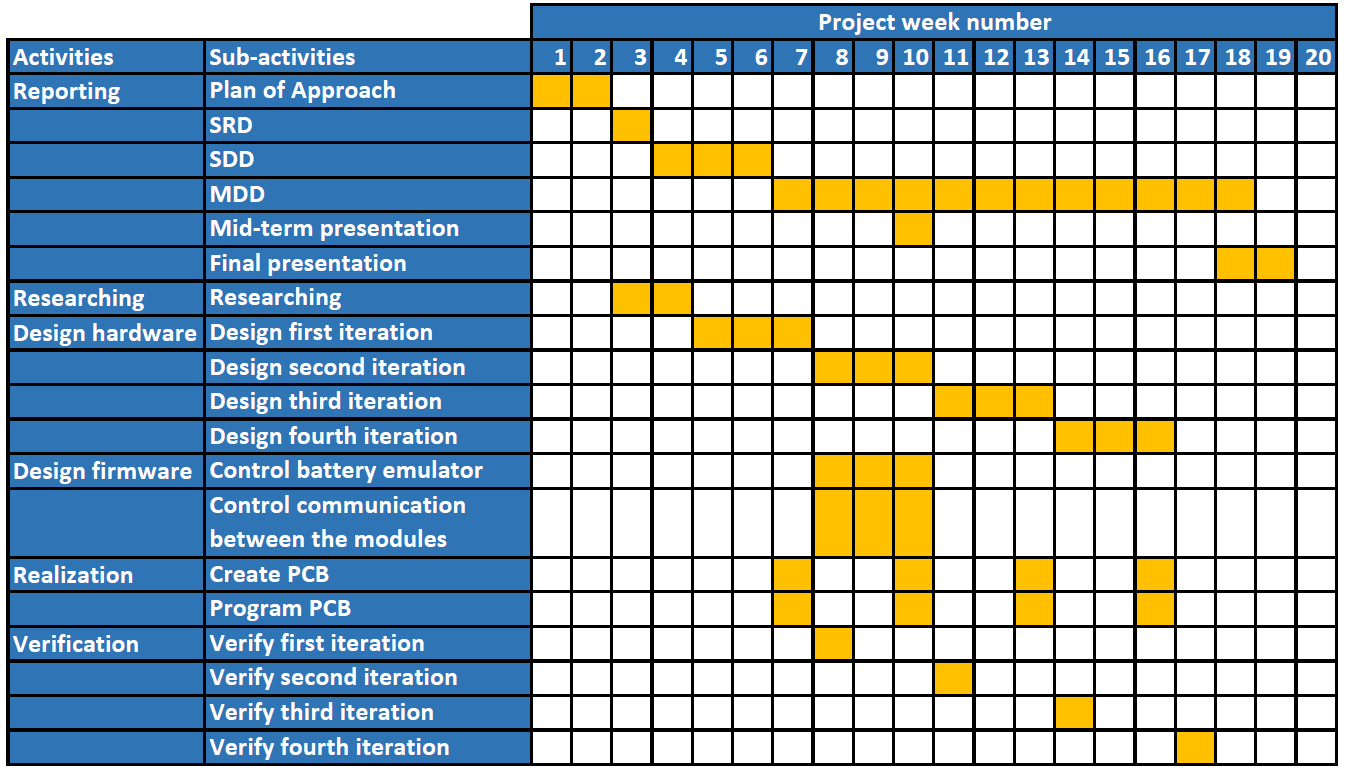
\includegraphics[width=\textwidth]{images/Broad_planning.png}
    \caption{planning}
    \label{tab:planning}
\end{figure}

% \begin{table}[ht!]
%     \begin{tabular}{lp{2.5in}|llllllllllllllllllll|}
%     \cline{3-22}
%                                                                            &                                                                            & \multicolumn{20}{c|}{\cellcolor[HTML]{00E2FF}\textbf{Project week number}}                                                                                                                                                                                                                                                                                                                                                                                                                                                                                                                                                                                                                                                                                                                                                                                                                                                                                                                                                                                                                                                                                          \\ \hline
%     \rowcolor[HTML]{00E2FF} 
%     \multicolumn{1}{|l|}{\cellcolor[HTML]{00E2FF}\textbf{Activities}}      & \textbf{Sub-activities}                                                    & \multicolumn{1}{l|}{\cellcolor[HTML]{00E2FF}\textbf{1}} & \multicolumn{1}{l|}{\cellcolor[HTML]{00E2FF}\textbf{2}} & \multicolumn{1}{l|}{\cellcolor[HTML]{00E2FF}\textbf{3}} & \multicolumn{1}{l|}{\cellcolor[HTML]{00E2FF}\textbf{4}} & \multicolumn{1}{l|}{\cellcolor[HTML]{00E2FF}\textbf{5}} & \multicolumn{1}{l|}{\cellcolor[HTML]{00E2FF}\textbf{6}} & \multicolumn{1}{l|}{\cellcolor[HTML]{00E2FF}\textbf{7}} & \multicolumn{1}{l|}{\cellcolor[HTML]{00E2FF}\textbf{8}} & \multicolumn{1}{l|}{\cellcolor[HTML]{00E2FF}\textbf{9}} & \multicolumn{1}{l|}{\cellcolor[HTML]{00E2FF}\textbf{10}} & \multicolumn{1}{l|}{\cellcolor[HTML]{00E2FF}\textbf{11}} & \multicolumn{1}{l|}{\cellcolor[HTML]{00E2FF}\textbf{12}} & \multicolumn{1}{l|}{\cellcolor[HTML]{00E2FF}\textbf{13}} & \multicolumn{1}{l|}{\cellcolor[HTML]{00E2FF}\textbf{14}} & \multicolumn{1}{l|}{\cellcolor[HTML]{00E2FF}\textbf{15}} & \multicolumn{1}{l|}{\cellcolor[HTML]{00E2FF}\textbf{16}} & \multicolumn{1}{l|}{\cellcolor[HTML]{00E2FF}\textbf{17}} & \multicolumn{1}{l|}{\cellcolor[HTML]{00E2FF}\textbf{18}} & \multicolumn{1}{l|}{\cellcolor[HTML]{00E2FF}\textbf{19}} & \textbf{20} \\ \hline
%     \multicolumn{1}{|l|}{\cellcolor[HTML]{00E2FF}\textbf{Reporting}}       & \cellcolor[HTML]{00E2FF}\textbf{Plan of Approach}                          & \multicolumn{1}{l|}{\cellcolor[HTML]{F8A102}}           & \multicolumn{1}{l|}{\cellcolor[HTML]{F8A102}}           & \multicolumn{1}{l|}{}                                   & \multicolumn{1}{l|}{}                                   & \multicolumn{1}{l|}{}                                   & \multicolumn{1}{l|}{}                                   & \multicolumn{1}{l|}{}                                   & \multicolumn{1}{l|}{}                                   & \multicolumn{1}{l|}{}                                   & \multicolumn{1}{l|}{}                                    & \multicolumn{1}{l|}{}                                    & \multicolumn{1}{l|}{}                                    & \multicolumn{1}{l|}{}                                    & \multicolumn{1}{l|}{}                                    & \multicolumn{1}{l|}{}                                    & \multicolumn{1}{l|}{}                                    & \multicolumn{1}{l|}{}                                    & \multicolumn{1}{l|}{}                                    & \multicolumn{1}{l|}{}                                    &             \\ \hline
%     \multicolumn{1}{|l|}{\cellcolor[HTML]{00E2FF}\textbf{}}                & \cellcolor[HTML]{00E2FF}\textbf{SRD}                                       & \multicolumn{1}{l|}{}                                   & \multicolumn{1}{l|}{}                                   & \multicolumn{1}{l|}{\cellcolor[HTML]{F8A102}}           & \multicolumn{1}{l|}{}                                   & \multicolumn{1}{l|}{}                                   & \multicolumn{1}{l|}{}                                   & \multicolumn{1}{l|}{}                                   & \multicolumn{1}{l|}{}                                   & \multicolumn{1}{l|}{}                                   & \multicolumn{1}{l|}{}                                    & \multicolumn{1}{l|}{}                                    & \multicolumn{1}{l|}{}                                    & \multicolumn{1}{l|}{}                                    & \multicolumn{1}{l|}{}                                    & \multicolumn{1}{l|}{}                                    & \multicolumn{1}{l|}{}                                    & \multicolumn{1}{l|}{}                                    & \multicolumn{1}{l|}{}                                    & \multicolumn{1}{l|}{}                                    &             \\ \hline
%     \multicolumn{1}{|l|}{\cellcolor[HTML]{00E2FF}\textbf{}}                & \cellcolor[HTML]{00E2FF}\textbf{SDD}                                       & \multicolumn{1}{l|}{}                                   & \multicolumn{1}{l|}{}                                   & \multicolumn{1}{l|}{}                                   & \multicolumn{1}{l|}{\cellcolor[HTML]{F8A102}}           & \multicolumn{1}{l|}{\cellcolor[HTML]{F8A102}}           & \multicolumn{1}{l|}{\cellcolor[HTML]{F8A102}}           & \multicolumn{1}{l|}{}                                   & \multicolumn{1}{l|}{}                                   & \multicolumn{1}{l|}{}                                   & \multicolumn{1}{l|}{}                                    & \multicolumn{1}{l|}{}                                    & \multicolumn{1}{l|}{}                                    & \multicolumn{1}{l|}{}                                    & \multicolumn{1}{l|}{}                                    & \multicolumn{1}{l|}{}                                    & \multicolumn{1}{l|}{}                                    & \multicolumn{1}{l|}{}                                    & \multicolumn{1}{l|}{}                                    & \multicolumn{1}{l|}{}                                    &             \\ \hline
%     \multicolumn{1}{|l|}{\cellcolor[HTML]{00E2FF}\textbf{}}                & \cellcolor[HTML]{00E2FF}\textbf{MDD / Research paper}                                       & \multicolumn{1}{l|}{}                                   & \multicolumn{1}{l|}{}                                   & \multicolumn{1}{l|}{}                                   & \multicolumn{1}{l|}{}                                   & \multicolumn{1}{l|}{}                                   & \multicolumn{1}{l|}{}                                   & \multicolumn{1}{l|}{\cellcolor[HTML]{F8A102}}           & \multicolumn{1}{l|}{\cellcolor[HTML]{F8A102}}           & \multicolumn{1}{l|}{\cellcolor[HTML]{F8A102}}           & \multicolumn{1}{l|}{\cellcolor[HTML]{F8A102}}            & \multicolumn{1}{l|}{\cellcolor[HTML]{F8A102}}            & \multicolumn{1}{l|}{\cellcolor[HTML]{F8A102}}            & \multicolumn{1}{l|}{\cellcolor[HTML]{F8A102}}            & \multicolumn{1}{l|}{\cellcolor[HTML]{F8A102}}            & \multicolumn{1}{l|}{\cellcolor[HTML]{F8A102}}            & \multicolumn{1}{l|}{\cellcolor[HTML]{F8A102}}            & \multicolumn{1}{l|}{\cellcolor[HTML]{F8A102}}            & \multicolumn{1}{l|}{\cellcolor[HTML]{F8A102}}            & \multicolumn{1}{l|}{}                                    &             \\ \hline
%     \multicolumn{1}{|l|}{\cellcolor[HTML]{00E2FF}\textbf{}}                & \cellcolor[HTML]{00E2FF}\textbf{Mid-term presentation}                     & \multicolumn{1}{l|}{}                                   & \multicolumn{1}{l|}{}                                   & \multicolumn{1}{l|}{}                                   & \multicolumn{1}{l|}{}                                   & \multicolumn{1}{l|}{}                                   & \multicolumn{1}{l|}{}                                   & \multicolumn{1}{l|}{}                                   & \multicolumn{1}{l|}{}                                   & \multicolumn{1}{l|}{}                                   & \multicolumn{1}{l|}{\cellcolor[HTML]{F8A102}}            & \multicolumn{1}{l|}{}                                    & \multicolumn{1}{l|}{}                                    & \multicolumn{1}{l|}{}                                    & \multicolumn{1}{l|}{}                                    & \multicolumn{1}{l|}{}                                    & \multicolumn{1}{l|}{}                                    & \multicolumn{1}{l|}{}                                    & \multicolumn{1}{l|}{}                                    & \multicolumn{1}{l|}{}                                    &             \\ \hline
%     \multicolumn{1}{|l|}{\cellcolor[HTML]{00E2FF}\textbf{}}                & \cellcolor[HTML]{00E2FF}\textbf{Final presentation}                        & \multicolumn{1}{l|}{}                                   & \multicolumn{1}{l|}{}                                   & \multicolumn{1}{l|}{}                                   & \multicolumn{1}{l|}{}                                   & \multicolumn{1}{l|}{}                                   & \multicolumn{1}{l|}{}                                   & \multicolumn{1}{l|}{}                                   & \multicolumn{1}{l|}{}                                   & \multicolumn{1}{l|}{}                                   & \multicolumn{1}{l|}{}                                    & \multicolumn{1}{l|}{}                                    & \multicolumn{1}{l|}{}                                    & \multicolumn{1}{l|}{}                                    & \multicolumn{1}{l|}{}                                    & \multicolumn{1}{l|}{}                                    & \multicolumn{1}{l|}{}                                    & \multicolumn{1}{l|}{}                                    & \multicolumn{1}{l|}{\cellcolor[HTML]{F8A102}}            & \multicolumn{1}{l|}{\cellcolor[HTML]{F8A102}}            &             \\ \hline
%     \multicolumn{1}{|l|}{\cellcolor[HTML]{00E2FF}\textbf{Researching}}     & \cellcolor[HTML]{00E2FF}\textbf{Researching}                               & \multicolumn{1}{l|}{}                                   & \multicolumn{1}{l|}{}                                   & \multicolumn{1}{l|}{\cellcolor[HTML]{F8A102}}           & \multicolumn{1}{l|}{\cellcolor[HTML]{F8A102}}           & \multicolumn{1}{l|}{}                                   & \multicolumn{1}{l|}{}                                   & \multicolumn{1}{l|}{}                                   & \multicolumn{1}{l|}{}                                   & \multicolumn{1}{l|}{}                                   & \multicolumn{1}{l|}{}                                    & \multicolumn{1}{l|}{}                                    & \multicolumn{1}{l|}{}                                    & \multicolumn{1}{l|}{}                                    & \multicolumn{1}{l|}{}                                    & \multicolumn{1}{l|}{}                                    & \multicolumn{1}{l|}{}                                    & \multicolumn{1}{l|}{}                                    & \multicolumn{1}{l|}{}                                    & \multicolumn{1}{l|}{}                                    &             \\ \hline
%     \multicolumn{1}{|l|}{\cellcolor[HTML]{00E2FF}\textbf{Design hardware}} & \cellcolor[HTML]{00E2FF}\textbf{Design first iteration}                    & \multicolumn{1}{l|}{}                                   & \multicolumn{1}{l|}{}                                   & \multicolumn{1}{l|}{}                                   & \multicolumn{1}{l|}{}                                   & \multicolumn{1}{l|}{\cellcolor[HTML]{F8A102}}           & \multicolumn{1}{l|}{\cellcolor[HTML]{F8A102}}           & \multicolumn{1}{l|}{\cellcolor[HTML]{F8A102}}           & \multicolumn{1}{l|}{\cellcolor[HTML]{F8A102}}           & \multicolumn{1}{l|}{\cellcolor[HTML]{F8A102}}           & \multicolumn{1}{l|}{}                                    & \multicolumn{1}{l|}{}                                    & \multicolumn{1}{l|}{}                                    & \multicolumn{1}{l|}{}                                    & \multicolumn{1}{l|}{}                                    & \multicolumn{1}{l|}{}                                    & \multicolumn{1}{l|}{}                                    & \multicolumn{1}{l|}{}                                    & \multicolumn{1}{l|}{}                                    & \multicolumn{1}{l|}{}                                    &             \\ \hline
%     \multicolumn{1}{|l|}{\cellcolor[HTML]{00E2FF}\textbf{}}                & \cellcolor[HTML]{00E2FF}\textbf{Design second iteration}                   & \multicolumn{1}{l|}{}                                   & \multicolumn{1}{l|}{}                                   & \multicolumn{1}{l|}{}                                   & \multicolumn{1}{l|}{}                                   & \multicolumn{1}{l|}{}                                   & \multicolumn{1}{l|}{}                                   & \multicolumn{1}{l|}{}                                   & \multicolumn{1}{l|}{}                                   & \multicolumn{1}{l|}{}                                   & \multicolumn{1}{l|}{\cellcolor[HTML]{F8A102}}            & \multicolumn{1}{l|}{\cellcolor[HTML]{F8A102}}            & \multicolumn{1}{l|}{\cellcolor[HTML]{F8A102}}            & \multicolumn{1}{l|}{}                                    & \multicolumn{1}{l|}{}                                    & \multicolumn{1}{l|}{}                                    & \multicolumn{1}{l|}{}                                    & \multicolumn{1}{l|}{}                                    & \multicolumn{1}{l|}{}                                    & \multicolumn{1}{l|}{}                                    &             \\ \hline
%     \multicolumn{1}{|l|}{\cellcolor[HTML]{00E2FF}\textbf{}}                & \cellcolor[HTML]{00E2FF}\textbf{Design third iteration}                    & \multicolumn{1}{l|}{}                                   & \multicolumn{1}{l|}{}                                   & \multicolumn{1}{l|}{}                                   & \multicolumn{1}{l|}{}                                   & \multicolumn{1}{l|}{}                                   & \multicolumn{1}{l|}{}                                   & \multicolumn{1}{l|}{}                                   & \multicolumn{1}{l|}{}                                   & \multicolumn{1}{l|}{}                                   & \multicolumn{1}{l|}{}                                    & \multicolumn{1}{l|}{}                                    & \multicolumn{1}{l|}{}                                    & \multicolumn{1}{l|}{\cellcolor[HTML]{F8A102}}            & \multicolumn{1}{l|}{}                                    & \multicolumn{1}{l|}{}                                    & \multicolumn{1}{l|}{}                                    & \multicolumn{1}{l|}{}                                    & \multicolumn{1}{l|}{}                                    & \multicolumn{1}{l|}{}                                    &             \\ \hline
%     \multicolumn{1}{|l|}{\cellcolor[HTML]{00E2FF}\textbf{}}                & \cellcolor[HTML]{00E2FF}\textbf{Design fourth iteration}                   & \multicolumn{1}{l|}{}                                   & \multicolumn{1}{l|}{}                                   & \multicolumn{1}{l|}{}                                   & \multicolumn{1}{l|}{}                                   & \multicolumn{1}{l|}{}                                   & \multicolumn{1}{l|}{}                                   & \multicolumn{1}{l|}{}                                   & \multicolumn{1}{l|}{}                                   & \multicolumn{1}{l|}{}                                   & \multicolumn{1}{l|}{}                                    & \multicolumn{1}{l|}{}                                    & \multicolumn{1}{l|}{}                                    & \multicolumn{1}{l|}{}                                    & \multicolumn{1}{l|}{\cellcolor[HTML]{F8A102}}            & \multicolumn{1}{l|}{\cellcolor[HTML]{F8A102}}            & \multicolumn{1}{l|}{\cellcolor[HTML]{F8A102}}            & \multicolumn{1}{l|}{}                                    & \multicolumn{1}{l|}{}                                    & \multicolumn{1}{l|}{}                                    &             \\ \hline
%     \multicolumn{1}{|l|}{\cellcolor[HTML]{00E2FF}\textbf{Design firmware}} & \cellcolor[HTML]{00E2FF}\textbf{Control battery emulator}                  & \multicolumn{1}{l|}{}                                   & \multicolumn{1}{l|}{}                                   & \multicolumn{1}{l|}{}                                   & \multicolumn{1}{l|}{}                                   & \multicolumn{1}{l|}{}                                   & \multicolumn{1}{l|}{}                                   & \multicolumn{1}{l|}{}                                   & \multicolumn{1}{l|}{\cellcolor[HTML]{F8A102}}           & \multicolumn{1}{l|}{\cellcolor[HTML]{F8A102}}           & \multicolumn{1}{l|}{\cellcolor[HTML]{F8A102}}            & \multicolumn{1}{l|}{}                                    & \multicolumn{1}{l|}{}                                    & \multicolumn{1}{l|}{}                                    & \multicolumn{1}{l|}{}                                    & \multicolumn{1}{l|}{}                                    & \multicolumn{1}{l|}{}                                    & \multicolumn{1}{l|}{}                                    & \multicolumn{1}{l|}{}                                    & \multicolumn{1}{l|}{}                                    &             \\ \hline
%     \multicolumn{1}{|l|}{\cellcolor[HTML]{00E2FF}\textbf{}}                & \cellcolor[HTML]{00E2FF}\textbf{Control communication between the modules} & \multicolumn{1}{l|}{}                                   & \multicolumn{1}{l|}{}                                   & \multicolumn{1}{l|}{}                                   & \multicolumn{1}{l|}{}                                   & \multicolumn{1}{l|}{}                                   & \multicolumn{1}{l|}{}                                   & \multicolumn{1}{l|}{}                                   & \multicolumn{1}{l|}{\cellcolor[HTML]{F8A102}}           & \multicolumn{1}{l|}{\cellcolor[HTML]{F8A102}}           & \multicolumn{1}{l|}{\cellcolor[HTML]{F8A102}}            & \multicolumn{1}{l|}{}                                    & \multicolumn{1}{l|}{}                                    & \multicolumn{1}{l|}{}                                    & \multicolumn{1}{l|}{}                                    & \multicolumn{1}{l|}{}                                    & \multicolumn{1}{l|}{}                                    & \multicolumn{1}{l|}{}                                    & \multicolumn{1}{l|}{}                                    & \multicolumn{1}{l|}{}                                    &             \\ \hline
%     \multicolumn{1}{|l|}{\cellcolor[HTML]{00E2FF}\textbf{Realization}}     & \cellcolor[HTML]{00E2FF}\textbf{Create PCB}                                & \multicolumn{1}{l|}{}                                   & \multicolumn{1}{l|}{}                                   & \multicolumn{1}{l|}{}                                   & \multicolumn{1}{l|}{}                                   & \multicolumn{1}{l|}{}                                   & \multicolumn{1}{l|}{}                                   & \multicolumn{1}{l|}{}                                   & \multicolumn{1}{l|}{}                                   & \multicolumn{1}{l|}{\cellcolor[HTML]{F8A102}}           & \multicolumn{1}{l|}{}                                    & \multicolumn{1}{l|}{}                                    & \multicolumn{1}{l|}{\cellcolor[HTML]{F8A102}}            & \multicolumn{1}{l|}{\cellcolor[HTML]{F8A102}}            & \multicolumn{1}{l|}{}                                    & \multicolumn{1}{l|}{}                                    & \multicolumn{1}{l|}{\cellcolor[HTML]{F8A102}}            & \multicolumn{1}{l|}{}                                    & \multicolumn{1}{l|}{}                                    & \multicolumn{1}{l|}{}                                    &             \\ \hline
%     \multicolumn{1}{|l|}{\cellcolor[HTML]{00E2FF}\textbf{}}                & \cellcolor[HTML]{00E2FF}\textbf{Program PCB}                               & \multicolumn{1}{l|}{}                                   & \multicolumn{1}{l|}{}                                   & \multicolumn{1}{l|}{}                                   & \multicolumn{1}{l|}{}                                   & \multicolumn{1}{l|}{}                                   & \multicolumn{1}{l|}{}                                   & \multicolumn{1}{l|}{}                                   & \multicolumn{1}{l|}{}                                   & \multicolumn{1}{l|}{\cellcolor[HTML]{F8A102}}           & \multicolumn{1}{l|}{}                                    & \multicolumn{1}{l|}{}                                    & \multicolumn{1}{l|}{\cellcolor[HTML]{F8A102}}            & \multicolumn{1}{l|}{\cellcolor[HTML]{F8A102}}            & \multicolumn{1}{l|}{}                                    & \multicolumn{1}{l|}{}                                    & \multicolumn{1}{l|}{\cellcolor[HTML]{F8A102}}            & \multicolumn{1}{l|}{}                                    & \multicolumn{1}{l|}{}                                    & \multicolumn{1}{l|}{}                                    &             \\ \hline
%     \multicolumn{1}{|l|}{\cellcolor[HTML]{00E2FF}\textbf{Verification}}    & \cellcolor[HTML]{00E2FF}\textbf{Verify first iteration}                    & \multicolumn{1}{l|}{}                                   & \multicolumn{1}{l|}{}                                   & \multicolumn{1}{l|}{}                                   & \multicolumn{1}{l|}{}                                   & \multicolumn{1}{l|}{}                                   & \multicolumn{1}{l|}{}                                   & \multicolumn{1}{l|}{}                                   & \multicolumn{1}{l|}{}                                   & \multicolumn{1}{l|}{}                                   & \multicolumn{1}{l|}{\cellcolor[HTML]{F8A102}}            & \multicolumn{1}{l|}{}                                    & \multicolumn{1}{l|}{}                                    & \multicolumn{1}{l|}{}                                    & \multicolumn{1}{l|}{}                                    & \multicolumn{1}{l|}{}                                    & \multicolumn{1}{l|}{}                                    & \multicolumn{1}{l|}{}                                    & \multicolumn{1}{l|}{}                                    & \multicolumn{1}{l|}{}                                    &             \\ \hline
%     \multicolumn{1}{|l|}{\cellcolor[HTML]{00E2FF}\textbf{}}                & \cellcolor[HTML]{00E2FF}\textbf{Verify second iteration}                   & \multicolumn{1}{l|}{}                                   & \multicolumn{1}{l|}{}                                   & \multicolumn{1}{l|}{}                                   & \multicolumn{1}{l|}{}                                   & \multicolumn{1}{l|}{}                                   & \multicolumn{1}{l|}{}                                   & \multicolumn{1}{l|}{}                                   & \multicolumn{1}{l|}{}                                   & \multicolumn{1}{l|}{}                                   & \multicolumn{1}{l|}{}                                    & \multicolumn{1}{l|}{}                                    & \multicolumn{1}{l|}{}                                    & \multicolumn{1}{l|}{\cellcolor[HTML]{F8A102}}            & \multicolumn{1}{l|}{}                                    & \multicolumn{1}{l|}{}                                    & \multicolumn{1}{l|}{}                                    & \multicolumn{1}{l|}{}                                    & \multicolumn{1}{l|}{}                                    & \multicolumn{1}{l|}{}                                    &             \\ \hline
%     \multicolumn{1}{|l|}{\cellcolor[HTML]{00E2FF}\textbf{}}                & \cellcolor[HTML]{00E2FF}\textbf{Verify third iteration}                    & \multicolumn{1}{l|}{}                                   & \multicolumn{1}{l|}{}                                   & \multicolumn{1}{l|}{}                                   & \multicolumn{1}{l|}{}                                   & \multicolumn{1}{l|}{}                                   & \multicolumn{1}{l|}{}                                   & \multicolumn{1}{l|}{}                                   & \multicolumn{1}{l|}{}                                   & \multicolumn{1}{l|}{}                                   & \multicolumn{1}{l|}{}                                    & \multicolumn{1}{l|}{}                                    & \multicolumn{1}{l|}{}                                    & \multicolumn{1}{l|}{}                                    & \multicolumn{1}{l|}{\cellcolor[HTML]{F8A102}}            & \multicolumn{1}{l|}{}                                    & \multicolumn{1}{l|}{}                                    & \multicolumn{1}{l|}{}                                    & \multicolumn{1}{l|}{}                                    & \multicolumn{1}{l|}{}                                    &             \\ \hline
%     \multicolumn{1}{|l|}{\cellcolor[HTML]{00E2FF}\textbf{}}                & \cellcolor[HTML]{00E2FF}\textbf{Verify fourth iteration}                   & \multicolumn{1}{l|}{}                                   & \multicolumn{1}{l|}{}                                   & \multicolumn{1}{l|}{}                                   & \multicolumn{1}{l|}{}                                   & \multicolumn{1}{l|}{}                                   & \multicolumn{1}{l|}{}                                   & \multicolumn{1}{l|}{}                                   & \multicolumn{1}{l|}{}                                   & \multicolumn{1}{l|}{}                                   & \multicolumn{1}{l|}{}                                    & \multicolumn{1}{l|}{}                                    & \multicolumn{1}{l|}{}                                    & \multicolumn{1}{l|}{}                                    & \multicolumn{1}{l|}{}                                    & \multicolumn{1}{l|}{}                                    & \multicolumn{1}{l|}{}                                    & \multicolumn{1}{l|}{\cellcolor[HTML]{F8A102}}            & \multicolumn{1}{l|}{}                                    & \multicolumn{1}{l|}{}                                    &             \\ \hline
%     \end{tabular}
%     \end{table}
\end{landscape}

\chapter{Cost-benefit overview}
	Since this project is part of the Dutch Battery research project BatteryNL,
additional budget and support are available. You will have access to experts
from the Centre of Expertise HRTech of the Hogeschool Rotterdam (HR) to
discuss technical findings and engineering choices to be made. They have a
battery testing setup that allows validation of battery models against actual
battery performance. You will also be in contact with fellow students from
HR who are working on a battery related project.

\chapter{Risk Analysis}
	%FILE FOR RISK ANALYSIS
There are many risks and reasons why the project might fail or go bad, A change in organizational priorities is the most common reason. A change in project objectives is also common as poor communication and unclear risk definition.
	\begin{itemize}
		\setlength\itemsep{-0.3em}
		\item Unclear or shifting goals.
		\item lack of planning.
		\item lack of follow up.
		\item timing issues 
		\item Lack of risk management.
		\item Unsuitable tools.
		\item Too many unsuitable tools
	\end{itemize}

\noindent
For this reason, table \ref{tab:risk_analysis} has been created with ratings that describe the probability of the project experiencing delays due to a specific reason and the corresponding impact. By multiplying these values together, a risk score is generated for each risk. To have a high chance of successfully completing the project, it is not acceptable for this score to be bigger then or equal to ten.

\newpage
\begin{table}[!h]
	\centering
	\begin{tabular}{|>{\columncolor{gray}}c|c|c|c|c|c|}
		\cline{2-6}
		\rowcolor{gray}
		\multicolumn{1}{l|}{\cellcolor{white}}&Very low&Low		&Medium					&High					&Very high 				\\ \hline
		Very likely	&\cellcolor{yellow}5&\cellcolor{orange}10	&\cellcolor{red}15		&\cellcolor{red}20		&\cellcolor{red}25 		\\ \hline
		likely		&\cellcolor{green}4	&\cellcolor{yellow}8	&\cellcolor{orange}12	&\cellcolor{red}16		&\cellcolor{red}20 		\\ \hline
		possible	&\cellcolor{green}3	&\cellcolor{yellow}6	&\cellcolor{yellow}9	&\cellcolor{orange}12	&\cellcolor{red}15 		\\ \hline
		Unlikely	&\cellcolor{green}2	&\cellcolor{green}4		&\cellcolor{yellow}6	&\cellcolor{yellow}8	&\cellcolor{orange}10	\\ \hline
		Rare		&\cellcolor{green}1	&\cellcolor{green}2		&\cellcolor{green}3		&\cellcolor{green}4		&\cellcolor{yellow}5	\\ \hline
	\end{tabular}
	\caption{risk analysis index}
\end{table}

\renewcommand\tabularxcolumn[1]{m{#1}}% for vertical centering text in X column

\begin{table}[!h]
	\begin{tabularx}{\textwidth}{|c|X|X|c|c|c|} \hline
		\# 	& Risk 													& Action 																				& Probability 	& Impact 	& Score 	\\ \hline
		1 	& A group member failed a deadline			            & The group member will be addressed by the group regarding this and will reasonably do everything in their power to rectify the situation. If this does not happen, the respective member may be removed from the project.										& 4	& 2			& \cellcolor{yellow}8	\\ \hline
		2 	& Messy file structure									& The version-controller looks after the structure of the folders						& 2	& 3			& \cellcolor{yellow}6	\\ \hline
		3 	& Behind planning for lack of knowledge or confusion	& Ask for help in time from fellow group members or teachers							& 2	& 3			& \cellcolor{yellow}6	\\ \hline
		4 	& There is insufficient communication in the group		& Weekly meetings where progress and tasks are discussed.								& 2	& 3			& \cellcolor{yellow}6	\\ \hline
		5 	& Clear results are missing								& The weekly meeting notes state clearly what activities have to be done the next week	& 1	& 3			& \cellcolor{green}3	\\ \hline
		6 	& Shortage in components								& Order parts early or look for available alternatives									& 2	& 4			& \cellcolor{yellow}8	\\ \hline
	\end{tabularx}
	\caption{Risk analysis}
	\label{tab:risk_analysis}
\end{table}

% Bibliography with heading so it pops up in the table of contents (i don't know why but this is how it works)
% \printbibliography[
% heading=bibintoc,
% title={Bibliography}
% ]
	\end{justify}
\end{document}
